%
% CHAPTER Versuch 1
%
\chapter{Aufnahme und Analyse eines Grauwertkeiles}
\label{chap:VERSUCH_1}
Dieser Abschnitt befasst sich mit der Aufnahme und Analyse eines Grauwertkeiles.
\section{Fragestellung, Messprinzip, Aufbau, Messmittel}
\label{chap:VERSUCH_1_FRAGESTELLUNG}
In diesem ersten Teil wird ein Bild eines Grauwertkeil mit Fünf Stufen aufgenommen. In diesem Fall sollten die einzelnen Graustufen in sich homogen sein, so das jeder Pixel, der diese Stufe ablichtet die selbe Helligkeit aufweisen sollte. In der Praxis ist dem aber nicht so, da verschiedene Störfaktoren eine Exakte Messung verhindern. Einige dieser Störungen sollen dann in den weiteren Versuchen behoben werden. Das Bild des Grauwertkeiles dient als Referenz, um die Effektivität der folgenden Korrekturmechanismen zu Bewerten. Wie bereits erwähnt liefert die Webcam Farbbilder, weshalb das aufgenommene Bild dann erst noch zu einem Schwarz/Weiß - Bild umgewandelt wird. Das Aufgenommene Bild wird dann in Fünf Unterbilder aufgeteilt, entsprechend den einzelnen Grausstufen. Von diesen Unterbildern wird dann der Mittelwert und die Standartabweichung der einzelnen Stufen berechnet. Diese dienen dann später als Referenz zum korrigierten Bild. Die Einstellungen der Belichtungsparameter der Kamera sind in allen Aufnahmen, während aller Versuche gleich und finden sich in Tabelle \ref{tab:BelichtungsParamter}


\begin{table}[H]
\centering
\begin{tabular}{l|c}
Parameter & Wert \\
\hline
frame height: & 480.0 \\
frame width: & 640.0 \\
\hline
brightness:  &  75.0 \\
contrast:    &  27.0 \\
saturation:  &  38.0\\
gain:        &  53.0\\
exposure:    &  -1.0\\
\hline
white balance: & 8986.0 \\
\hline
distance to object: & 32.4 cm \\
\end{tabular}
\caption{Belichtungsparameter der Webcam}
\label{tab:BelichtungsParamter}
\end{table}


Die entsprechenden Standartabweichungen wurden folgendermaßen berechnet.
\begin{equation}
s = \sqrt{\frac{1}{n-1}\sum_{i=1}^{n} (p_i- \bar{p})^2}
\end{equation}
Dabei ist $n$ gerade die Gesamtanzahl an Pixeln über die die Standartabweichung $s$ berechnet werden soll und $\bar{p}$ der Durchschnitt aller Pixel über diesen Bereich.

\section{Messwerte}
\label{chap:VERSUCH_1_MESSWERTE}
\begin{figure}[H]
\centering
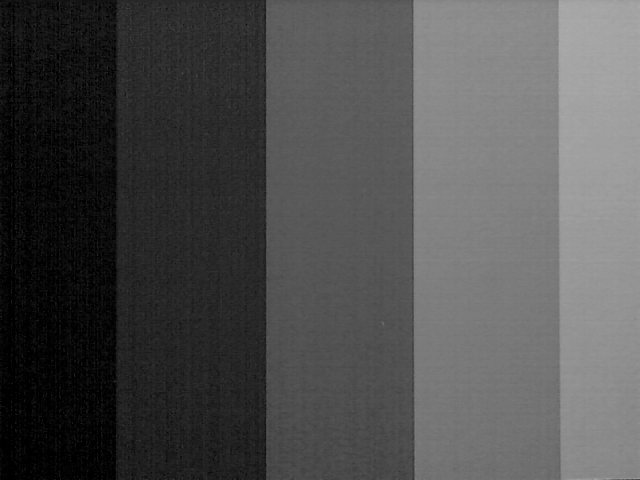
\includegraphics[width=150mm]{graustufen.png}
\caption{Grauwertkeil}
\label{img:Grauwertkeil}
\end{figure}
\begin{table}
\centering
\begin{tabular}{c|cc}
Stufe & Durchschnitt & Standardabweichung \\
\hline
1 & 9.3699 & 7.4903 \\
2 & 39.1486 & 5.9921 \\
3 & 85.7785 & 6.9256 \\
4 & 126.9901 & 8.8584 \\
5 & 152.3874 & 9.1518 \\
\end{tabular}
\caption{Durchschnitt und Standartabweichung der Graustufen in sich.}
\label{tab:GrauStufen_Mean}
\end{table}
\section{Auswertung und Interpretation}
\label{chap:VERSUCH_1_AUSWERTUNG}
Die Ergebnisse der Mittelwertsberechung entspricht den Erwartungen. Auch die Standartabweichung verhält sich nicht ausergewöhnlich.
Der Durchschnitt für den schwarzen Bereich des Bildes ist unter dem ersten Tabelleneintrag zu finden. Der Durchschnitt für den hellsten Teil des Bildes unter dem letzen Tabelleneintrag. Tabelle \ref{tab:GrauStufen_Mean} Mit diesen Werten wird später das korrigierte Bild verglichen, um die effektivität der Kalibrierung zu überprüfen.
